\documentclass[12pt]{article}
\usepackage[russian]{babel}
\usepackage[utf8x]{inputenc}
\usepackage{amssymb}
\usepackage{amsmath}
\usepackage{graphicx}
\usepackage{geometry}
\usepackage[colorinlistoftodos]{todonotes}
\usepackage{listings}
\usepackage[section]{placeins}
\begin{document}

\title{3. Реализация быстрого преобразования Фурье}
\author{Андрей Валиков}
\date{}
\maketitle
																																																								\section{Математическая модель сигнала}

\noindent Константы имеют следующие значения:
\[f_1 = 1000\]
\[A_{f_1} = 0.5\]
\[\varphi_1 = 120\]

\[f_2 = 3000\]
\[A_{f_2} = 1\]
\[\varphi_2 = 180\]

\[f_3 = 6000\]
\[A_{f_3} = 5\]
\[\varphi_3 = 90\]

По ним вычисляется значение исходного сигнала:
\[x(t) = \sum_{k = 1}^{3} A_{f_k}\sin(2\pi f_k t + \varphi_k)\]

\begin{lstlisting}
def Func(t):
  A   = [    1,      2,    10]
  f   = [10000,  20000, 40000]
  Phi = [.5236, 2.0944, .7854]

  y = 0
  for k in range(3):
    y += A[k] * np.sin(t * np.pi * f[k] + Phi[k])
  return y
\end{lstlisting}

\begin{figure}[!htb]
\centering
%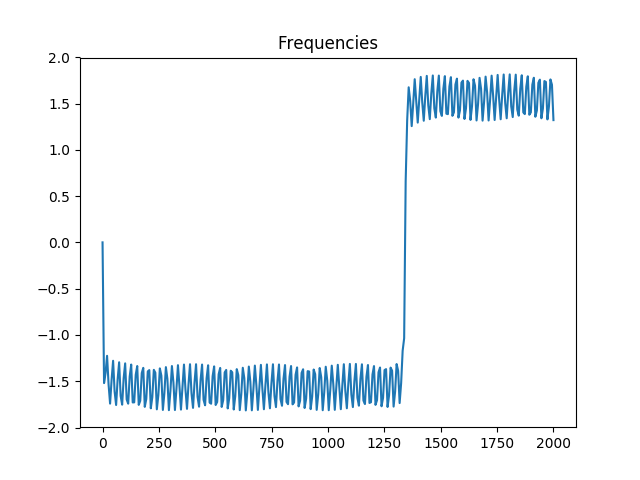
\includegraphics[scale=1.00]{frequencies.png}
\caption{}
\label{}
\end{figure}

\begin{figure}[htp]
\centering
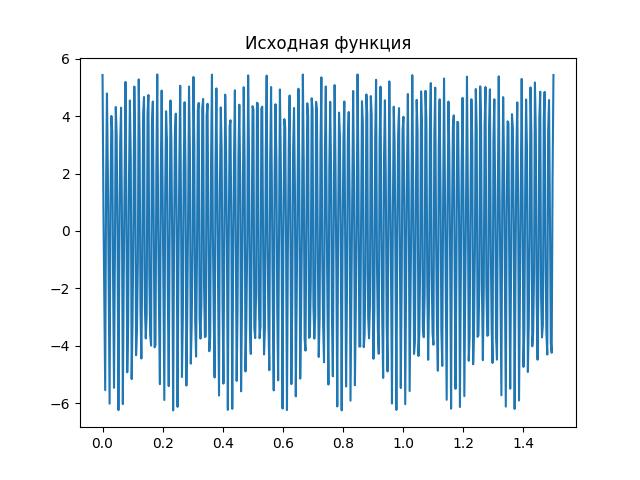
\includegraphics[scale=1.00]{origin.png}
\caption{}
\label{}
\end{figure}

\section{Вычисление дискретного преобразованния Фурье}
Формула:

\[X(t)=\sum_{n=0}^{N-1}x(n)e^{-2\pi nki / N}\]
 


\begin{lstlisting}
import numpy as np

def dft_exp(k, n, N):
  return np.exp((-1j * 2 * np.pi * n * k) / N)
\end{lstlisting}

\begin{figure}[!htb]
\centering
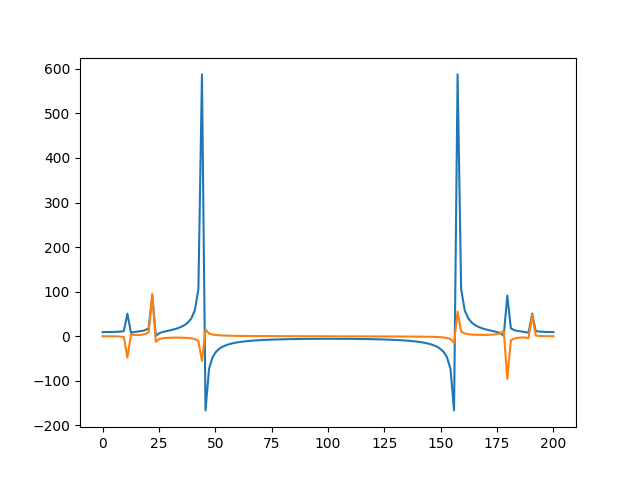
\includegraphics[scale=1.00]{func_dft.png}
\caption{}
\label{}
\end{figure}



\section{Вычисление быстрого преобразованния Фурье}

%\[f(\frac{1}{\pi} \int_{0}^{\infty}(\operatorname{Re}(\hat{f})\cos(\omega t) - \operatorname{Im}(\hat{f})\sin(\omega t))d\omega \]

\begin{lstlisting}
import numpy as np
from dft_part import dft_exp


def FFT(X):

  N = len(X)
  V = np.log2(N)

  if V % 2 != 0:
    V = np.ceil(V)
    AddN = 2 ** V - N
    X = np.concatenate([X, np.zeros(int(AddN))])
    N = len(X)

  y = []

  if N == 2:
    y.append(X[0] + X[1])
    y.append(X[0] - X[1])
    return y
  
  else:
    E  = np.zeros(N // 2)
    O  = np.zeros(N // 2)

    Ek = 0
    Ok = 0

    for k in range(N):

      if k % 2 == 0:
        E[Ek] = X[k]
        Ek += 1

      else:
        O[Ok] = X[k]
        Ok += 1

    X1 = FFT(E)
    X2 = FFT(O)

    for k in range(N):
      if k < N / 2:
        y.append(X1[k] + dft_exp(k, 1, N) * X2[k])
      
      else:
        y.append(X1[k - N // 2] - dft_exp(k - N // 2, 1, N) * X2[k - N // 2])

    return y
\end{lstlisting}

\begin{figure}[!htb]
\centering
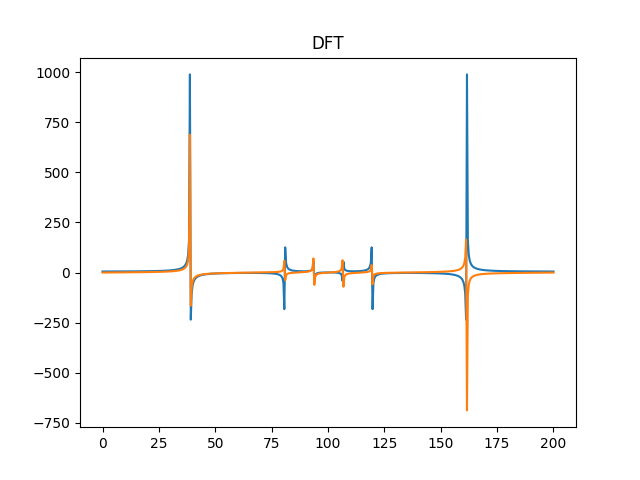
\includegraphics[scale=1.00]{dft.png}
\caption{}
\label{}


\end{figure}

\section{Функция ошибки}
\begin{figure}[htp]
\centering
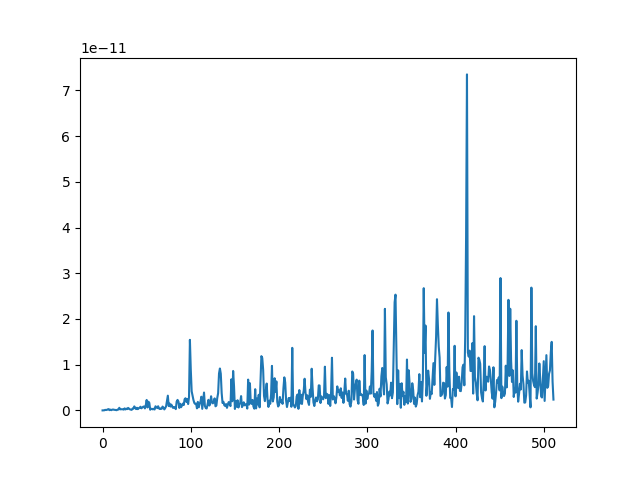
\includegraphics[scale=1.00]{err.png}
\caption{}
\label{}
\end{figure}

\section{Вывод}
Имеется исходная полигармоническая функция. В работе сравнивается скорость и точность дискретного и быстрого преобразований Фурье. По формуле дисккретного преобразования Фурье (исходное значение умноженное на поворотный множитель). В быстром преобразовании Фурье значительно сокращается количество вычислительно сложной операции умножения. Функция ошибки показывает максимальное отклонение около $10^{-11}$, что говорит о высокой точности. Скорость также намного выше.

\end{document}